% Options for packages loaded elsewhere
\PassOptionsToPackage{unicode}{hyperref}
\PassOptionsToPackage{hyphens}{url}
%
\documentclass[
]{book}
\usepackage{amsmath,amssymb}
\usepackage{iftex}
\ifPDFTeX
  \usepackage[T1]{fontenc}
  \usepackage[utf8]{inputenc}
  \usepackage{textcomp} % provide euro and other symbols
\else % if luatex or xetex
  \usepackage{unicode-math} % this also loads fontspec
  \defaultfontfeatures{Scale=MatchLowercase}
  \defaultfontfeatures[\rmfamily]{Ligatures=TeX,Scale=1}
\fi
\usepackage{lmodern}
\ifPDFTeX\else
  % xetex/luatex font selection
\fi
% Use upquote if available, for straight quotes in verbatim environments
\IfFileExists{upquote.sty}{\usepackage{upquote}}{}
\IfFileExists{microtype.sty}{% use microtype if available
  \usepackage[]{microtype}
  \UseMicrotypeSet[protrusion]{basicmath} % disable protrusion for tt fonts
}{}
\makeatletter
\@ifundefined{KOMAClassName}{% if non-KOMA class
  \IfFileExists{parskip.sty}{%
    \usepackage{parskip}
  }{% else
    \setlength{\parindent}{0pt}
    \setlength{\parskip}{6pt plus 2pt minus 1pt}}
}{% if KOMA class
  \KOMAoptions{parskip=half}}
\makeatother
\usepackage{xcolor}
\usepackage{color}
\usepackage{fancyvrb}
\newcommand{\VerbBar}{|}
\newcommand{\VERB}{\Verb[commandchars=\\\{\}]}
\DefineVerbatimEnvironment{Highlighting}{Verbatim}{commandchars=\\\{\}}
% Add ',fontsize=\small' for more characters per line
\usepackage{framed}
\definecolor{shadecolor}{RGB}{248,248,248}
\newenvironment{Shaded}{\begin{snugshade}}{\end{snugshade}}
\newcommand{\AlertTok}[1]{\textcolor[rgb]{0.94,0.16,0.16}{#1}}
\newcommand{\AnnotationTok}[1]{\textcolor[rgb]{0.56,0.35,0.01}{\textbf{\textit{#1}}}}
\newcommand{\AttributeTok}[1]{\textcolor[rgb]{0.13,0.29,0.53}{#1}}
\newcommand{\BaseNTok}[1]{\textcolor[rgb]{0.00,0.00,0.81}{#1}}
\newcommand{\BuiltInTok}[1]{#1}
\newcommand{\CharTok}[1]{\textcolor[rgb]{0.31,0.60,0.02}{#1}}
\newcommand{\CommentTok}[1]{\textcolor[rgb]{0.56,0.35,0.01}{\textit{#1}}}
\newcommand{\CommentVarTok}[1]{\textcolor[rgb]{0.56,0.35,0.01}{\textbf{\textit{#1}}}}
\newcommand{\ConstantTok}[1]{\textcolor[rgb]{0.56,0.35,0.01}{#1}}
\newcommand{\ControlFlowTok}[1]{\textcolor[rgb]{0.13,0.29,0.53}{\textbf{#1}}}
\newcommand{\DataTypeTok}[1]{\textcolor[rgb]{0.13,0.29,0.53}{#1}}
\newcommand{\DecValTok}[1]{\textcolor[rgb]{0.00,0.00,0.81}{#1}}
\newcommand{\DocumentationTok}[1]{\textcolor[rgb]{0.56,0.35,0.01}{\textbf{\textit{#1}}}}
\newcommand{\ErrorTok}[1]{\textcolor[rgb]{0.64,0.00,0.00}{\textbf{#1}}}
\newcommand{\ExtensionTok}[1]{#1}
\newcommand{\FloatTok}[1]{\textcolor[rgb]{0.00,0.00,0.81}{#1}}
\newcommand{\FunctionTok}[1]{\textcolor[rgb]{0.13,0.29,0.53}{\textbf{#1}}}
\newcommand{\ImportTok}[1]{#1}
\newcommand{\InformationTok}[1]{\textcolor[rgb]{0.56,0.35,0.01}{\textbf{\textit{#1}}}}
\newcommand{\KeywordTok}[1]{\textcolor[rgb]{0.13,0.29,0.53}{\textbf{#1}}}
\newcommand{\NormalTok}[1]{#1}
\newcommand{\OperatorTok}[1]{\textcolor[rgb]{0.81,0.36,0.00}{\textbf{#1}}}
\newcommand{\OtherTok}[1]{\textcolor[rgb]{0.56,0.35,0.01}{#1}}
\newcommand{\PreprocessorTok}[1]{\textcolor[rgb]{0.56,0.35,0.01}{\textit{#1}}}
\newcommand{\RegionMarkerTok}[1]{#1}
\newcommand{\SpecialCharTok}[1]{\textcolor[rgb]{0.81,0.36,0.00}{\textbf{#1}}}
\newcommand{\SpecialStringTok}[1]{\textcolor[rgb]{0.31,0.60,0.02}{#1}}
\newcommand{\StringTok}[1]{\textcolor[rgb]{0.31,0.60,0.02}{#1}}
\newcommand{\VariableTok}[1]{\textcolor[rgb]{0.00,0.00,0.00}{#1}}
\newcommand{\VerbatimStringTok}[1]{\textcolor[rgb]{0.31,0.60,0.02}{#1}}
\newcommand{\WarningTok}[1]{\textcolor[rgb]{0.56,0.35,0.01}{\textbf{\textit{#1}}}}
\usepackage{longtable,booktabs,array}
\usepackage{calc} % for calculating minipage widths
% Correct order of tables after \paragraph or \subparagraph
\usepackage{etoolbox}
\makeatletter
\patchcmd\longtable{\par}{\if@noskipsec\mbox{}\fi\par}{}{}
\makeatother
% Allow footnotes in longtable head/foot
\IfFileExists{footnotehyper.sty}{\usepackage{footnotehyper}}{\usepackage{footnote}}
\makesavenoteenv{longtable}
\usepackage{graphicx}
\makeatletter
\def\maxwidth{\ifdim\Gin@nat@width>\linewidth\linewidth\else\Gin@nat@width\fi}
\def\maxheight{\ifdim\Gin@nat@height>\textheight\textheight\else\Gin@nat@height\fi}
\makeatother
% Scale images if necessary, so that they will not overflow the page
% margins by default, and it is still possible to overwrite the defaults
% using explicit options in \includegraphics[width, height, ...]{}
\setkeys{Gin}{width=\maxwidth,height=\maxheight,keepaspectratio}
% Set default figure placement to htbp
\makeatletter
\def\fps@figure{htbp}
\makeatother
\setlength{\emergencystretch}{3em} % prevent overfull lines
\providecommand{\tightlist}{%
  \setlength{\itemsep}{0pt}\setlength{\parskip}{0pt}}
\setcounter{secnumdepth}{5}
\usepackage{booktabs}
\ifLuaTeX
  \usepackage{selnolig}  % disable illegal ligatures
\fi
\usepackage[]{natbib}
\bibliographystyle{plainnat}
\IfFileExists{bookmark.sty}{\usepackage{bookmark}}{\usepackage{hyperref}}
\IfFileExists{xurl.sty}{\usepackage{xurl}}{} % add URL line breaks if available
\urlstyle{same}
\hypersetup{
  pdftitle={Theory-driven analysis of ecological data: a practical handbook},
  pdfauthor={us},
  hidelinks,
  pdfcreator={LaTeX via pandoc}}

\title{Theory-driven analysis of ecological data: a practical handbook}
\author{us}
\date{2024-03-14}

\usepackage{amsthm}
\newtheorem{theorem}{Theorem}[chapter]
\newtheorem{lemma}{Lemma}[chapter]
\newtheorem{corollary}{Corollary}[chapter]
\newtheorem{proposition}{Proposition}[chapter]
\newtheorem{conjecture}{Conjecture}[chapter]
\theoremstyle{definition}
\newtheorem{definition}{Definition}[chapter]
\theoremstyle{definition}
\newtheorem{example}{Example}[chapter]
\theoremstyle{definition}
\newtheorem{exercise}{Exercise}[chapter]
\theoremstyle{definition}
\newtheorem{hypothesis}{Hypothesis}[chapter]
\theoremstyle{remark}
\newtheorem*{remark}{Remark}
\newtheorem*{solution}{Solution}
\begin{document}
\maketitle

{
\setcounter{tocdepth}{1}
\tableofcontents
}
\chapter{About Bookdown}\label{about-bookdown}

This is a \emph{sample} book written in \textbf{Markdown}. You can use anything that Pandoc's Markdown supports; for example, a math equation \(a^2 + b^2 = c^2\).

\section{Usage}\label{usage}

Each \textbf{bookdown} chapter is an .Rmd file, and each .Rmd file can contain one (and only one) chapter. A chapter \emph{must} start with a first-level heading: \texttt{\#\ A\ good\ chapter}, and can contain one (and only one) first-level heading.

Use second-level and higher headings within chapters like: \texttt{\#\#\ A\ short\ section} or \texttt{\#\#\#\ An\ even\ shorter\ section}.

The \texttt{index.Rmd} file is required, and is also your first book chapter. It will be the homepage when you render the book.

\section{Render book}\label{render-book}

You can render the HTML version of this example book without changing anything:

\begin{enumerate}
\def\labelenumi{\arabic{enumi}.}
\item
  Find the \textbf{Build} pane in the RStudio IDE, and
\item
  Click on \textbf{Build Book}, then select your output format, or select ``All formats'' if you'd like to use multiple formats from the same book source files.
\end{enumerate}

Or build the book from the R console:

\begin{Shaded}
\begin{Highlighting}[]
\NormalTok{bookdown}\SpecialCharTok{::}\FunctionTok{render\_book}\NormalTok{()}
\end{Highlighting}
\end{Shaded}

To render this example to PDF as a \texttt{bookdown::pdf\_book}, you'll need to install XeLaTeX. You are recommended to install TinyTeX (which includes XeLaTeX): \url{https://yihui.org/tinytex/}.

\section{Preview book}\label{preview-book}

As you work, you may start a local server to live preview this HTML book. This preview will update as you edit the book when you save individual .Rmd files. You can start the server in a work session by using the RStudio add-in ``Preview book'', or from the R console:

\begin{Shaded}
\begin{Highlighting}[]
\NormalTok{bookdown}\SpecialCharTok{::}\FunctionTok{serve\_book}\NormalTok{()}
\end{Highlighting}
\end{Shaded}

\section{Here are some useful things for writing the book using bookdown}\label{here-are-some-useful-things-for-writing-the-book-using-bookdown}

All chapters start with a first-level heading followed by your chapter title, like the line above. There should be only one first-level heading (\texttt{\#}) per .Rmd file.

\subsection{A section}\label{a-section}

All chapter sections start with a second-level (\texttt{\#\#}) or higher heading followed by your section title, like the sections above and below here. You can have as many as you want within a chapter.

\subsubsection*{An unnumbered section}\label{an-unnumbered-section}
\addcontentsline{toc}{subsubsection}{An unnumbered section}

Chapters and sections are numbered by default. To un-number a heading, add a \texttt{\{.unnumbered\}} or the shorter \texttt{\{-\}} at the end of the heading, like in this section.

\section{Cross-references}\label{cross}

Cross-references make it easier for your readers to find and link to elements in your book.

\subsection{Chapters and sub-chapters}\label{chapters-and-sub-chapters}

There are two steps to cross-reference any heading:

\begin{enumerate}
\def\labelenumi{\arabic{enumi}.}
\tightlist
\item
  Label the heading: \texttt{\#\ Hello\ world\ \{\#nice-label\}}.

  \begin{itemize}
  \tightlist
  \item
    Leave the label off if you like the automated heading generated based on your heading title: for example, \texttt{\#\ Hello\ world} = \texttt{\#\ Hello\ world\ \{\#hello-world\}}.
  \item
    To label an un-numbered heading, use: \texttt{\#\ Hello\ world\ \{-\#nice-label\}} or \texttt{\{\#\ Hello\ world\ .unnumbered\}}.
  \end{itemize}
\item
  Next, reference the labeled heading anywhere in the text using \texttt{\textbackslash{}@ref(nice-label)}; for example, please see Chapter \ref{cross}.

  \begin{itemize}
  \tightlist
  \item
    If you prefer text as the link instead of a numbered reference use: \hyperref[cross]{any text you want can go here}.
  \end{itemize}
\end{enumerate}

\subsection{Captioned figures and tables}\label{captioned-figures-and-tables}

Figures and tables \emph{with captions} can also be cross-referenced from elsewhere in your book using \texttt{\textbackslash{}@ref(fig:chunk-label)} and \texttt{\textbackslash{}@ref(tab:chunk-label)}, respectively.

See Figure \ref{fig:nice-fig}.

\begin{Shaded}
\begin{Highlighting}[]
\FunctionTok{par}\NormalTok{(}\AttributeTok{mar =} \FunctionTok{c}\NormalTok{(}\DecValTok{4}\NormalTok{, }\DecValTok{4}\NormalTok{, .}\DecValTok{1}\NormalTok{, .}\DecValTok{1}\NormalTok{))}
\FunctionTok{plot}\NormalTok{(pressure, }\AttributeTok{type =} \StringTok{\textquotesingle{}b\textquotesingle{}}\NormalTok{, }\AttributeTok{pch =} \DecValTok{19}\NormalTok{)}
\end{Highlighting}
\end{Shaded}

\begin{figure}

{\centering 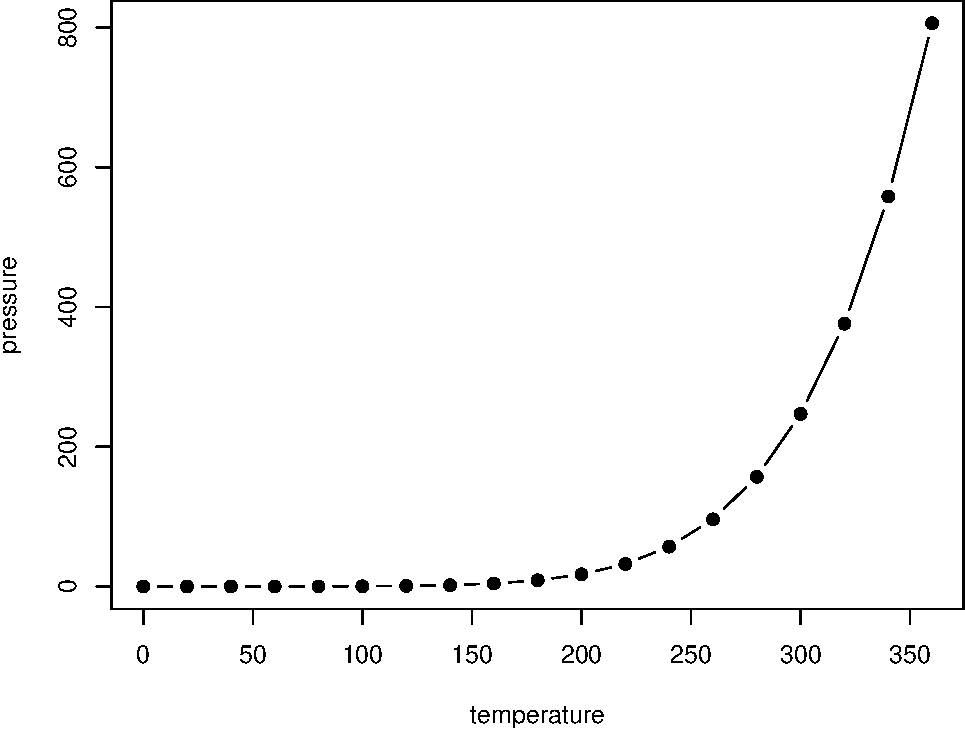
\includegraphics[width=0.8\linewidth]{_main_files/figure-latex/nice-fig-1} 

}

\caption{Here is a nice figure!}\label{fig:nice-fig}
\end{figure}

Don't miss Table \ref{tab:nice-tab}.

\begin{Shaded}
\begin{Highlighting}[]
\NormalTok{knitr}\SpecialCharTok{::}\FunctionTok{kable}\NormalTok{(}
  \FunctionTok{head}\NormalTok{(pressure, }\DecValTok{10}\NormalTok{), }\AttributeTok{caption =} \StringTok{\textquotesingle{}Here is a nice table!\textquotesingle{}}\NormalTok{,}
  \AttributeTok{booktabs =} \ConstantTok{TRUE}
\NormalTok{)}
\end{Highlighting}
\end{Shaded}

\begin{table}

\caption{\label{tab:nice-tab}Here is a nice table!}
\centering
\begin{tabular}[t]{rr}
\toprule
temperature & pressure\\
\midrule
0 & 0.0002\\
20 & 0.0012\\
40 & 0.0060\\
60 & 0.0300\\
80 & 0.0900\\
\addlinespace
100 & 0.2700\\
120 & 0.7500\\
140 & 1.8500\\
160 & 4.2000\\
180 & 8.8000\\
\bottomrule
\end{tabular}
\end{table}

\section{Parts}\label{parts}

You can add parts to organize one or more book chapters together. Parts can be inserted at the top of an .Rmd file, before the first-level chapter heading in that same file.

Add a numbered part: \texttt{\#\ (PART)\ Act\ one\ \{-\}} (followed by \texttt{\#\ A\ chapter})

Add an unnumbered part: \texttt{\#\ (PART\textbackslash{}*)\ Act\ one\ \{-\}} (followed by \texttt{\#\ A\ chapter})

Add an appendix as a special kind of un-numbered part: \texttt{\#\ (APPENDIX)\ Other\ stuff\ \{-\}} (followed by \texttt{\#\ A\ chapter}). Chapters in an appendix are prepended with letters instead of numbers.

\section{Footnotes and citations}\label{footnotes-and-citations}

\subsection{Footnotes}\label{footnotes}

Footnotes are put inside the square brackets after a caret \texttt{\^{}{[}{]}}. Like this one \footnote{This is a footnote.}.

\subsection{Citations}\label{citations}

Reference items in your bibliography file(s) using \texttt{@key}.

For example, we are using the \textbf{bookdown} package \citep{R-bookdown} (check out the last code chunk in index.Rmd to see how this citation key was added) in this sample book, which was built on top of R Markdown and \textbf{knitr} \citep{xie2015} (this citation was added manually in an external file book.bib).
Note that the \texttt{.bib} files need to be listed in the index.Rmd with the YAML \texttt{bibliography} key.

The RStudio Visual Markdown Editor can also make it easier to insert citations: \url{https://rstudio.github.io/visual-markdown-editing/\#/citations}

\section{Blocks}\label{blocks}

\subsection{Equations}\label{equations}

Here is an equation.

\begin{equation} 
  f\left(k\right) = \binom{n}{k} p^k\left(1-p\right)^{n-k}
  \label{eq:binom}
\end{equation}

You may refer to using \texttt{\textbackslash{}@ref(eq:binom)}, like see Equation \eqref{eq:binom}.

\subsection{Theorems and proofs}\label{theorems-and-proofs}

Labeled theorems can be referenced in text using \texttt{\textbackslash{}@ref(thm:tri)}, for example, check out this smart theorem \ref{thm:tri}.

\begin{theorem}
\protect\hypertarget{thm:tri}{}\label{thm:tri}For a right triangle, if \(c\) denotes the \emph{length} of the hypotenuse
and \(a\) and \(b\) denote the lengths of the \textbf{other} two sides, we have
\[a^2 + b^2 = c^2\]
\end{theorem}

Read more here \url{https://bookdown.org/yihui/bookdown/markdown-extensions-by-bookdown.html}.

\subsection{Callout blocks}\label{callout-blocks}

The R Markdown Cookbook provides more help on how to use custom blocks to design your own callouts: \url{https://bookdown.org/yihui/rmarkdown-cookbook/custom-blocks.html}

\section{Sharing your book}\label{sharing-your-book}

\subsection{Publishing}\label{publishing}

HTML books can be published online, see: \url{https://bookdown.org/yihui/bookdown/publishing.html}

\subsection{404 pages}\label{pages}

By default, users will be directed to a 404 page if they try to access a webpage that cannot be found. If you'd like to customize your 404 page instead of using the default, you may add either a \texttt{\_404.Rmd} or \texttt{\_404.md} file to your project root and use code and/or Markdown syntax.

\subsection{Metadata for sharing}\label{metadata-for-sharing}

Bookdown HTML books will provide HTML metadata for social sharing on platforms like Twitter, Facebook, and LinkedIn, using information you provide in the \texttt{index.Rmd} YAML. To setup, set the \texttt{url} for your book and the path to your \texttt{cover-image} file. Your book's \texttt{title} and \texttt{description} are also used.

This \texttt{gitbook} uses the same social sharing data across all chapters in your book- all links shared will look the same.

Specify your book's source repository on GitHub using the \texttt{edit} key under the configuration options in the \texttt{\_output.yml} file, which allows users to suggest an edit by linking to a chapter's source file.

Read more about the features of this output format here:

\url{https://pkgs.rstudio.com/bookdown/reference/gitbook.html}

Or use:

\begin{Shaded}
\begin{Highlighting}[]
\NormalTok{?bookdown}\SpecialCharTok{::}\NormalTok{gitbook}
\end{Highlighting}
\end{Shaded}

\chapter{Preambule}\label{preambule}

Who is the textbook for?

\chapter{Why mathematical models? (Sonia)}\label{why-mathematical-models-sonia}

\section{Big data}\label{big-data}

According to IBM, every day humanity generates 2.5 trillion (2.5 billion billion) bytes of text, image and sound data (\url{https://www-01.ibm.com/software/fr/data/bigdata}). Acceleration of information accumulation. We can learn from massive amount of data available.

When read by machines (analyses, they can reveal a wealth of unsuspected correlations (or that are difficult to identify). Success of Amazon or Netflix at learning what you like from studying your habits.

Machine learning (ML), a subset of AI that enables computers to learn from training data, has been highly effective at predicting various types of cancer, including breast, brain, lung, liver, and prostate cancer. In fact, AI and ML have demonstrated greater accuracy in predicting cancer than clinicians.

So, knowledge can emerge from this data analysis (even without any idea of the underlying laws).

This lead some people to suggest that we may not need theory anymore (``The end of theory: the data deluge, Wired). The availability of data and the development of methods to analyse them: does they mean that we're going through a major epistemological change? In other terms: do we still need models and theory?

\url{https://www.ncbi.nlm.nih.gov/pmc/articles/PMC2711825/}

\section{What is theory?}\label{what-is-theory}

We define \emph{ecological theory} broadly as an explanation of an ecological phenomenon. These explanations take the form of narratives that explain how an ecological process works, or why an ecological pattern is observed, and that becomes scientifically useful when expressed in a logical structure (Pickett et al.~2010; Rossberg et al.~2019).

Maris et al.~2017: ``Scientific theories contain universal or general propositions regarding the system in question; they generally encompass a set of models, or rules to build models, as representations of the properties and dynamics of target systems. Models can then be expressed as hypotheses within a formal framework (van Fraassen 1980, Giere 2004).''

The transformation of an idea in narrative form into a logical, testable theory often, though not always, involves the use of \emph{models} (Otto and Rosales 2020).

\section{What's a model?}\label{whats-a-model}

\url{https://en.wikipedia.org/wiki/Ecosystem_model}

The concept of a model is derived from scale models, referring to simplified replicas of larger structures such as, for instance, buildings or ships. This implies a structural similarity between a model and its original. Thus, \textbf{models are idealized representations of certain aspects of our study systems. They are idealized versions of reality}, just as architectural models represent key features of complex structures and model organisms represent a group of organisms that share common attributes (Kokko 2007).

Models can be as simple as a verbal statement about a subject or two boxes connected by an arrow to represent some relationship (conceptual models). Alternatively, models can be extremely complex and detailed, such as a mathematical description of the pathways of nitrogen transformations within ecosystems.

A mathematical model can be an equation or a set of equations (mathematical expressions) that describes how different aspects of a system relate to one another (Otto and Day 2007). They can be phenomenological or mechanistic (Grainger et al.~2022).

Theory and math are not inexorably linked. Indeed, many excellent theories do not involve math (e.g., the theory of evolution by natural selection; Darwin 1859), and many uses of math in ecology are not theory (e.g., practical applications of statistics).

Because models are an idealized, simplified version of the real world (e.g.~maps), they are therefore not real. They're incomplete, they're wrong (intro Kokko's book).
\textbf{``all models are false but some models are useful''}
\url{https://en.wikipedia.org/wiki/All_models_are_wrong}

The systems we're interested in are complex. How can we hope capturing the complexity of reality? We can't.
And if we did, it would not be helpful (if models are as complex as reality, e.g.~map) because of:

\begin{itemize}
\tightlist
\item
  too many parameters to measure (would require too much time and resources),
\item
  the equations are insoluble and require too long to run on even a good computer,
\item
  even if soluble, we might not be able to understand the results.
\end{itemize}

\textbf{Modeling involves a choice about what to include and what to leave out.}
We need to simplify systems in a way that preserves the essential features of the system (depending on our interest). This means that our big task as modelers is to decide what goes in the model and what doesn't. The art of modeling is to decide which aspect of reality one can sacrifice and which ones are crucial to retain.

We want to work with manageable models which max generality, realism and precision towards the goals of understanding and predicting\ldots.

These goals typically compete with each other so real models are mathematical descriptions that result from tradeoffs among these goals which depend on our needs: the tension between realism, generality, and precision:
\textbf{Levins 1966}
\url{https://v4.chriskrycho.com/2016/realism-generality-and-precision-in-tension.html}

\begin{itemize}
\item
  One can sacrifice generality to realism and precision. E.g. fisheries; good measurement of shot-time behavior, numerical solution, precise testable predictions applicable to a particular situation).
\item
  One can sacrifice realism to generality and precision. E.g. physics-like models (general equations such as LV). The way in which nature deviates from theory will indicate where further complexity will be useful.
\item
  One can sacrifice precision to realism and generality. E.g. MacArthur 1965. People concerned with the qualitative behavior (not quantitative). Graphical models.
\end{itemize}

\section{Purpose of science?}\label{purpose-of-science}

Understand and predict.

\section{Can we do that with big data (data analysis?)}\label{can-we-do-that-with-big-data-data-analysis}

Big data analysis reveals correlations. (Again, this can be useful)
But those correlations are not causal.
Famous examples of spurious correlations.
Correlations can emerge by chance because you look at some many variables.
Correlations can happen because of confounding factors, e.g.~the example of shoe size and level of math in a school (due to age)

So we can find correlations, but we often don't know why. So we can't understand (understanding is finding associations that are causal).

This does not mean that non-causal correlations can't help predict! They can have great predictive power. Amazon, Netflix.
So we can learn from those data and their analysis, even without causal knowledge.

We can predict, but we can also fail at predicting. Predictions can fail because lacks of general rules, so extrapolations can fail; financial crisis, elections. It relies on what happened in the past, so unable to work in new situations.

Predict without understanding\ldots. act without understanding? Risks (cf justice, police, discriminations)

Big data don't create theory, they need it to be exploited. (This last statement could evolve in the future? In particular, new analyses methods suggest they can successfully retrive causality from correlations; cg Zach, Stan's paper with Correlation Cross mapping).

Because of that, we can argue that we still do need theory and models! (models are one langage of theory, one way of expressing it)

\section{The scientific method}\label{the-scientific-method}

Let's step back and reflect on the process by which science is carried out. The \emph{scientific method} is an empirical method for acquiring knowledge that has characterized the development of science since at least the 17th century.

Science (through the scientific method) can build on previous knowledge and develop a more sophisticated understanding of its topics of study over time.

\begin{itemize}
\item
  \textbf{`Problem' identification}: It involves careful observation which leads to the formulation of a question.
\item
  \textbf{Hypothesis}: A hypothesis is a conjecture (hypothetical explanations), based on the observation/the knowledge obtained while formulating the question, that may explain any given behavior. A scientific hypothesis must be falsifiable, implying that it is possible to identify a possible outcome of an experiment or observation that conflicts with predictions deduced from the hypothesis; otherwise, the hypothesis cannot be meaningfully tested.
  Falsifiability is a deductive standard of evaluation of scientific theories and hypotheses, introduced by the philosopher of science Karl Popper in his book The Logic of Scientific Discovery (1934).
  A theory or hypothesis is falsifiable (or refutable) if it can be logically contradicted by an empirical test.
\item
  \textbf{Prediction}: The prediction step deduces the logical consequences of the hypothesis before the outcome is known.
\item
  \textbf{Testing}: Hypotheses are tested by conducting experiments or gathering observations. The purpose of the test is to determine whether observations agree with or conflict with the expectations deduced from a hypothesis.
\item
  \textbf{Refinement (or elimination) of the hypotheses} based on the experimental findings.
\end{itemize}

Although procedures vary from one field of inquiry to another, the underlying process is frequently the same. In sum, the process is as follows: making conjectures (hypotheses), deriving predictions from them as logical consequences, and then carrying out experiments based on those predictions to determine whether the original conjecture was correct.

\textbf{The scientific method is an iterative, cyclical process through which information is continually revised.}

\section{A feedback loop involving data and models}\label{a-feedback-loop-involving-data-and-models}

A scientific understanding of the biological world arises when ideas about how nature works are formalized, tested, refined, and then tested again.

\textbf{Scientific inquiry should operate as a feedback loop} in which theory that describes the natural world is developed, tested empirically through carefully articulated hypotheses, modified to better represent reality, and then tested again.

When this feedback loop works, \textbf{theory} provides a framework to guide inquiry, experimental design, and the interpretation of observed patterns, supplies mathematical tools to harness information from collected data, and connects individual experiments to general ideas about how nature operates.

In turn, \textbf{empirical research} can be used to support, refute, or revise theoretical predictions, indicate which theoretical assumptions are consistent with the natural world, and point theoreticians to overlooked processes that can be integrated into models.

\textbf{However, there is currently a disconnection between theoretical and empirical research.}

Although the benefits of feedback between theoretical and empirical research are widely acknowledged by ecologists, this link is still not as strong as it could be in ecological research.

Indeed, up to 45\% of articles on empirical ecology make no mention of any theory whatsoever (Scheiner 2013), and fewer than 10\% of ecologists and evolutionary biologists agree with the statement that `theoretical findings drive empirical work' in their fields (Haller 2014).

Further references about the disconnect between empirical and theoretical work in ecology: Lomnicki 1988; Kareiva 1989; Fawcett and Higginson 2012; Scheiner 2013; Haller 2014; Rossberg et al.~2019.

\textbf{Why this disconnection?}

\begin{itemize}
\tightlist
\item
  A lack of theoretical training in ecology (Rossberg et al.~2019).
\item
  A lack of motivation on the part of some theoreticians to engage with the language of empiricists (Grimm 1994) or with the elements of nature that empiricists focus on (Krebs 1988).
\item
  A general lack of mutual appreciation between empiricists and theoreticians (Haller 2014).
\item
  Persistent communication barriers between these two groups (Servedio 2020), in particular that theory is expressed in the langage of math (some ecologists may not have formal background in math and theoretical papers may not be written with a general audience, not always explaining asumptions, terminology and notations), some aspects of the theory may seem inaccessible by some, the more equations an ecology and evolutionary biology article contains, the fewer citations it receives (Fawcett and Higginson 2012).
\end{itemize}

This barrier presents a major challenge to the full integration of theoretical and empirical work in ecology.

\textbf{A better integration of theory into empirical work is needed} (Caswell 1988; Pickett et al.~2010; Marquet et al.~2014; Servedio et al.~2014; Servedio 2020).

This is especially important in the context of global change.

This is why this course/book!

\chapter{What types of theoretical models in ecology? (Isa)}\label{what-types-of-theoretical-models-in-ecology-isa}

\section{What system? What question? What hypotheses (no maths shown here)}\label{what-system-what-question-what-hypotheses-no-maths-shown-here}

\begin{itemize}
\tightlist
\item
  Question is related to a specific level of organization / scale and determine what can be ignored
\item
  Examples of questions for each scale based on our recurrent example plant-herbivore (P-H)
\item
  Updated Levin's triangle illustrated by different (P-H) with related questions =\textgreater{} define variables
\item
  What can be ignored? Upper level is slower than lower ones and its dynamics may be ignored
\item
  Link between assumptions, model and predictions, with the risk of overinterpretation
\item
  The different types of assumptions (critical, exploratory, logistical)
\item
  Illustration of assumption types with the Grazing-optimisation example
\end{itemize}

\section{What model formalism? (no maths shown here)}\label{what-model-formalism-no-maths-shown-here}

\subsection{Deterministic -- stochastic processes}\label{deterministic-stochastic-processes}

\begin{itemize}
\tightlist
\item
  What does stochasticity come from? Environmental, demographic, trait variability
\item
  When should we account for it (illustration with pop logistic growth (no math) with addition or not of gaussian noise)

  \begin{itemize}
  \tightlist
  \item
    for questions related to output variability
  \item
    when output distribution is skewed and mean no more a good predictor (small pop)
  \end{itemize}
\item
  When can we use deterministic: when processes can be summarised with averaged parameters
\item
  NB: mention of master equations (deterministic equation summarising stochastic model)
\end{itemize}

\subsection{Time: discrete -- continuous}\label{time-discrete-continuous}

How do the processes are structured along time? when using discrete vs continuous time

\begin{itemize}
\tightlist
\item
  Discrete-time:

  \begin{itemize}
  \tightlist
  \item
    Fixed generation times
  \item
    Synchronization of processes (e.g., seasonal forcing)
  \item
    Sequential processes with specific order (e.g., complex life-cycle) =\textgreater{} more transparent
  \end{itemize}
\item
  Continuous time:

  \begin{itemize}
  \tightlist
  \item
    Events can happen at any time
  \item
    Generation overlap
  \end{itemize}
\item
  Illustration with logistic pop growth in continuous and discrete time:

  \begin{itemize}
  \tightlist
  \item
    discrete-time with small ∆t boils down to continuous
  \item
    discrete time have richer dynamics due to a lag
  \end{itemize}
\item
  Both can be either stochastic or deterministic
\end{itemize}

\subsection{Accounting for space}\label{accounting-for-space}

\begin{itemize}
\tightlist
\item
  None vs spatial:

  \begin{itemize}
  \tightlist
  \item
    TIB, example of space implicit; In none spatial models, space is assumed homogenous and the scale can be defined with the units (example: pop density in ind/km2)
  \item
    When does the question need it? Are spatial processes impacting local dynamics of interest or are we interested in patterns emerging at higher spatial scale from local processes? Implicit vs Explicit: does geographical positions matter or only topology?
  \end{itemize}
\item
  Topology versus Distances explicit

  \begin{itemize}
  \tightlist
  \item
    Topology (metapop model): space is represented in the structure of space and strength of connectivity. Adapted to study fragmented landscapes or problems related to structure of connectivity
  \item
    Explicit: distances are explicit; in 1 (Fisher KPP) or two dimensions (grid): adapted to represents fronts, gradients, edge effects; or if interested with emerging spatial patterns
  \end{itemize}
\item
  Discrete within the distance explicit case: grids vs Continuous (PDE):

  \begin{itemize}
  \tightlist
  \item
    Continuous adapted to model processes occurring progressing locally (diffusion) but not processes with large distance / heterogeneous effects
  \item
    Grids with small mesh size can boil down to continuous (sometimes, discretisation is used for a technical approximation of continuous space) =\textgreater{} question of technical relevance.
  \item
    As continuous can be more difficult (math) this can prevent its use (mention of lab heritage)
  \end{itemize}
\end{itemize}

\section{What technical choices?}\label{what-technical-choices}

\subsection{Analytical -- Numerical}\label{analytical-numerical}

\begin{itemize}
\tightlist
\item
  What do we gain in making models simple? =\textgreater{} Principle of parcimony

  \begin{itemize}
  \tightlist
  \item
    Analytical solution: we know the state of the model at any time point given
  \item
    Tractable model: We are able to express equilibrium with parameters and study local stability =\textgreater{} we can say generalities about the long term dynamics
  \item
    Intractable models: we are obliged to do simulations using approximations (numerical algorithm or integration); the results depend on the parameter values and initial conditions.
  \item
    The dimension of the parameter space to explore is exponentially linked to the number of parameters
  \item
    Simulations allow to investigate transient dynamics
  \end{itemize}
\end{itemize}

\subsection{Rules versus Maths}\label{rules-versus-maths}

\begin{itemize}
\tightlist
\item
  What is an agent-based model? Algorithm which represent processes with a series of rules applied to each agent at each time step using proba: example with birth, death, interactions
\item
  What is the alternative: Math =\textgreater{} equations: example of ODE, SDE, DE, PDE: what does it mean?

  \begin{itemize}
  \tightlist
  \item
    ODE: change over time of our variable of interest (SDE; with some stochasticity)
  \item
    DE: State at the next time step
  \item
    PDE: Change over time and space
  \end{itemize}
\item
  Advantages / Disadvantages:

  \begin{itemize}
  \tightlist
  \item
    ABM:

    \begin{itemize}
    \tightlist
    \item
      The dynamics emerge from elemental processes
    \item
      Simpler to build from empirical knowledge
    \item
      But high computation consumption
    \item
      Rarely tractable
    \end{itemize}
  \item
    Equations

    \begin{itemize}
    \tightlist
    \item
      Use of math and approximation for simplifications
    \item
      Have large analysis power for extreme cases
    \item
      Fast computation
    \item
      Easier to fit to data
    \item
      The relations between variables are imposed: processes synthetized
    \end{itemize}
  \end{itemize}
\item
  To what questions / system/ conditions is it most adapted?

  \begin{itemize}
  \tightlist
  \item
    ABM:

    \begin{itemize}
    \tightlist
    \item
      When stochastic processes are dominant (ex: conservation of small pops)
    \item
      When there are no too many parameters
    \item
      For some questions where processes are difficult to synthesise (behaviour)
    \item
      When there is no math skills around!
    \end{itemize}
  \item
    Equations:

    \begin{itemize}
    \tightlist
    \item
      Whenever processes can be synthesised with average parameters
    \item
      =\textgreater{} Large populations
    \end{itemize}
  \end{itemize}
\end{itemize}

\section{Some classical models used in ecology and seen next days}\label{some-classical-models-used-in-ecology-and-seen-next-days}

\begin{itemize}
\tightlist
\item
  Systems of differential equations, no space :

  \begin{itemize}
  \tightlist
  \item
    Verhulst (logistic growth), Lotka-Volterra predator-prey (Day 2)
  \item
    Lotka-Volterra, food web niche model (Day 4)
  \end{itemize}
\item
  Spatial systems of differential equations: TIB, Levins' occupancy (Day3)
\item
  Spatial IBM: Neutral model of biodiversity from Hubbel (Day 3)
\end{itemize}

A Rmarkdown file will be available to provide the code of the illustrations of section 2.2

\chapter{How to build a model? (Isa)}\label{how-to-build-a-model-isa}

(1h) Lecture with interactivity (and Rmarkdown file for some parts)

\begin{itemize}
\tightlist
\item
  I will present different pictures of different plant-herbivore systems with associated research questions and ask how they will sketch the system (on board) to do a mode.
\item
  I will ask then which formalism they would choose and why (in terms of determinism, time, space) {[}and we can try writing rules or equations?{]}
\item
  Then we will focus on a question for which the Rosenzweig-MacArthur model (ODE) is appropriate, I will write the model on board and ask all the assumptions they could see that are behind the model formulation. We will discuss in which regards they are appropriate for our question.
\item
  Then we will study line by line a code in R to explain how this could be implemented in R, while also explaining the principle of numerical integration.
\item
  I will let them 5-10min to run the model and plot some dynamics and ask them how they would use it to answer the question (to introduce the next section).
\end{itemize}

\chapter{How to analyze a model? (Isa)}\label{how-to-analyze-a-model-isa}

(1h) Interactive lecture + based on a script for some parts

(Rmarkdown file with the example of Rosenzweig-MacArthur model)

\begin{itemize}
\item
  Analyze the behavior of the model long-term (Box 3 Grainger et al AmNat)

  \begin{itemize}
  \tightlist
  \item
    Local stability (when possible for long term dynamics) (script)

    \begin{itemize}
    \tightlist
    \item
      Calculating equilibria
    \item
      What are the Jacobian matrix and eigenvalues (meaning but no math derivation) ?
    \item
      How to interpret the eigenvalues to infer the long term behavior type
    \end{itemize}
  \end{itemize}
\item
  Isoclines / graphical
  *Phase plane (script)
\item
  Bifurcation diagrams (long term dynamics) (script)
\item
  When results depend on initial conditions =\textgreater{} finding all the equilibria of intractable ODE systems (loop to run large series of initial conditions, function searchZeros of package nleqslv)
\item
  Model Usages to answer the question (will try to show some concrete examples of questions to answer with these usages for the model of section 3a)

  \begin{itemize}
  \tightlist
  \item
    Parameter variation (see bifurcation diagrams + example DeMaz Grazing-Optimization)
  \item
    Comparison with a null model to assess the impact of a process (with or without the process, with different formulation of the process. Example with functional responses (script)
  \item
    Generation of synthetic data on which to run in silico experiments. - Example of food webs under different regimes of perturbations.
  \end{itemize}
\item
  Parameter exploration and robustness of conclusions

  \begin{itemize}
  \tightlist
  \item
    Exhaustivity is possible (tractable)
  \item
    We know the values of parameters from empirical data =\textgreater{} allows us to fix or restrain the range of some parameters.
  \item
    Sensitivity analysis: effect size when varying 10\% each parameter + look if conclusions are modified if the most sensitive parameters are varied.
  \end{itemize}
\end{itemize}

  \bibliography{book.bib,packages.bib}

\end{document}
